% TO-DO:
% * 立法机制
% * 

\documentclass[10pt]{beamer}

\usepackage[CJKspace]{xeCJK}
% \setCJKmainfont[BoldFont=Alibaba PuHuiTi Bold,ItalicFont=AR PL KaitiM GB]{Alibaba PuHuiTi Light}
\setCJKmainfont[ItalicFont=AR PL KaitiM GB]{Alibaba PuHuiTi}
\setmainfont[ItalicFont=Latin Modern Roman Slanted]{Alibaba Sans:style=Light}

%\usepackage{newtxtext,newtxmath}	% use Times Roman font
\usepackage{newtxtext}
\renewcommand{\familydefault}{\sfdefault}
%\usefonttheme{serif}
\usefonttheme{professionalfonts}
%\setbeamertemplate{theorems}[numbered]
\setbeamertemplate{caption}{\insertcaption} 	% no `Figure' prefix before caption

\mode<presentation> {

%\usetheme{default}
%\usetheme{AnnArbor}
%\usetheme{Antibes}
%\usetheme{Bergen}
%\usetheme{Berkeley}
%\usetheme{Berlin}
%\usetheme{Boadilla}
%\usetheme{CambridgeUS}
%\usetheme{Copenhagen}
%\usetheme{Darmstadt}
\usetheme{Dresden}
%\usetheme{Frankfurt}
%\usetheme{Goettingen}
%\usetheme{Hannover}
%\usetheme{Ilmenau}
%\usetheme{JuanLesPins}
%\usetheme{Luebeck}
%\usetheme{Madrid}
%\usetheme{Malmoe}
%\usetheme{Marburg}
%\usetheme{Montpellier}
%\usetheme{PaloAlto}
%\usetheme{Pittsburgh}
%\usetheme{Rochester}
%\usetheme{Singapore}
%\usetheme{Szeged}
%\usetheme{Warsaw}

%\usecolortheme{albatross}
%\usecolortheme{beaver}
%\usecolortheme{beetle}
%\usecolortheme{crane}
%\usecolortheme{dolphin}
%\usecolortheme{dove}
%\usecolortheme{fly}
%\usecolortheme{lily}
%\usecolortheme{orchid}
%\usecolortheme{rose}
%\usecolortheme{seagull}
%\usecolortheme{seahorse}
%\usecolortheme{whale}
\usecolortheme{wolverine}

%\setbeamertemplate{footline} % To remove the footer line in all slides uncomment this line
\setbeamertemplate{footline}[page number] % To replace the footer line in all slides with a simple slide count uncomment this line
\setbeamertemplate{navigation symbols}{} % To remove the navigation symbols from the bottom of all slides uncomment this line
}

\setbeamertemplate{headline}{}
\setbeamersize{text margin left=1mm,text margin right=4mm} 
%\settowidth{\leftmargini}{\usebeamertemplate{itemize item}}
%\addtolength{\leftmargini}{\labelsep}

\usepackage[backend=biber,style=numeric]{biblatex}
\bibliography{../AGI-book}
\bibliography{../Economics}
\renewcommand*{\bibfont}{\footnotesize}
\setbeamertemplate{bibliography item}[text]

\usepackage{graphicx} % Allows including images
\usepackage{tikz-cd}
% \usepackage{ulem}
\usepackage[export]{adjustbox}% http://ctan.org/pkg/adjustbox
\usepackage{verbatim} % comments
% \usepackage{tikz-cd}  % commutative diagrams
% \newcommand{\tikzmark}[1]{\tikz[overlay,remember picture] \node (#1) {};}
% \usepackage{booktabs} % Allows the use of \toprule, \midrule and \bottomrule in tables
% \usepackage{amssymb}  % \leftrightharpoons
\usepackage{wasysym} % frownie face
\usepackage{newtxtext,newtxmath}	% Times New Roman font

\newcommand{\emp}[1]{{\color{blue}#1}}
\newcommand{\vect}[1]{\boldsymbol{#1}}
\newcommand{\tab}{\hspace*{1cm}}
\newcommand*\confoundFace{$\vcenter{\hbox{
\includegraphics[scale=0.2]{../confounded-face.jpg}}}$}
\renewcommand{\smiley}{$\vcenter{\hbox{
\includegraphics[scale=0.05]{../smiling-face.png}}}$}

%%%%%%%% Make table of contents %%%%%%%

\makeatletter
\renewcommand{\boxed}[1]{\fbox{\m@th$\displaystyle\scalebox{0.9}{#1}$} \,}
\makeatother
\newif\ifframeinlbf
\frameinlbftrue
\makeatletter
\newcommand\listofframes{\@starttoc{lbf}}
\makeatother

\addtobeamertemplate{frametitle}{}{%
	\ifframeinlbf
	\addcontentsline{lbf}{section}{\protect\makebox[2em][l]{%
			\protect\usebeamercolor[fg]{structure}\insertframenumber\hfill}%
		\insertframetitle\par}%
	\else\fi
}

%----------------------------------------------------------------------------------------
%	TITLE PAGE
%----------------------------------------------------------------------------------------

\title[HK neutral party]{\Huge《香港中立派》}
\author{HK.neutrality@gmail.com}
%\author{\cc{YKY 甄景贤}{YKY}} % Your name
%\institute[] % Your institution as it will appear on the bottom of every slide, may be shorthand to save space
%{
%Independent researcher, Hong Kong \\ % Your institution for the title page
%\medskip
%\textit{generic.intelligence@gmail.com} % Your email address
%}
\date{\today} % Date, can be changed to a custom date

\begin{document}

\frameinlbffalse
\usebackgroundtemplate{%
	\begin{picture}(0,278)
	
\includegraphics[width=\paperwidth]{HK-2.png}
	\end{picture}}
\addtocounter{page}{-1}
\begin{frame}[plain,noframenumbering]
\titlepage
\end{frame}

\usebackgroundtemplate{}
\addtocounter{page}{-1}
\begin{frame}[noframenumbering]
\frametitle{Table of contents}
\listofframes
\vspace*{0.5cm}
政綱 与 基本思想 如下,但仍會不斷 修正 和 改進

多谢 各界支持 \smiley
\end{frame}

%----------------------------------------------------------------------------------------
%	PRESENTATION SLIDES
%----------------------------------------------------------------------------------------

%------------------------------------------------

\frameinlbftrue
\begin{frame}
\frametitle{民主/普选制度 是倒退的,妨礙进步}

\begin{itemize}
	\item 一人一票的民主制度,令社会不断 回归到平均值,这对於技术发达的西方国家,或许并无大碍,但香港仍处於技术相对落后的后殖民主义阶段,在发展中地区的政治形势更严峻,更需要建立 \emp{meritocracy}

	\item 西方历史上,民主的发源地 希腊雅典,亦没有因为有民主而免於战败。 民主的 Athens 被 Sparta 打败,即著名的 Pelopponesian War
	
	\item 柏拉图、亚里士多德 等哲学家 提出 政治的 \emp{循环} (cycle): \\
	\begin{tikzcd}[ampersand replacement=\&,arrows=Rightarrow,row sep=0em,column sep=small]
		\mbox{mob rule} \arrow{r} \& \mbox{monarchy} \arrow{r} \& \mbox{tyranny} \arrow[d,bend left=90] \\
		\mbox{democracy} \arrow[u,bend left=90] \& \arrow{l} \mbox{oligarchy} \& \arrow{l} \mbox{aristocracy}
	\end{tikzcd} \\
	% \tab mob rule $\Rightarrow$ monarchy $\Rightarrow$ tyranny $\Rightarrow$ aristocracy $\Rightarrow$ oligarchy $\Rightarrow$ democracy $\Rightarrow$ mob rule
	民主只是其中一個 不穩定的 階段

	\item 美国 开国国父们都不喜欢民主,例如 John Adams 说: \textit{民主比 贵族 和 独裁 更血腥,一样 虚伪、自私 和 贪婪,而且必然会 自我毁灭}

	\item 「中国模式」令中国近10-20年经济起飞,一定做对了某些事。 它似乎证明了民主对於经济进步是不必要的。 印度有民主,但经济一样 起唔到飞

	\item 中国 在不平等条约下割让香港; 中英联合声明 在历史上发挥了平稳过渡的功能,但它承诺的 选举制度,其实不利进步
	\end{itemize}
\end{frame}

\begin{frame}
\frametitle{香港人的民族自卑感}
\begin{itemize}
	\item 亚洲年轻人 的幼稚化,原因之一是 科技上无法追上欧美,导致强烈的出卖同胞欲望(宁愿做狗不做人)
	
	% \item 「揽炒」是一些读书唔成的学生,希望别人也无法返校,非常可鄙

	\item 必需积极地在 本地 和国际上 消除种族歧视,亚洲人才有希望过有尊严的生活

	\item 种族歧视 的解药,并不是 反向种族歧视,而是 \emp{消除}种族歧视
	
	\item 香港中立的优点可以吸引世界上 支持 种族平等 的人材 来港,而不是 吸引一班 racist「鬼佬」来港 坐享特权

	\item 有些人觉得 普选 + 三权分立 就是完美的政治制度,其实只是 100\% 照抄美国,缺乏独立思考
	
	\item 而美国的民主制逐渐演变成 两党制,选 Bush 也是打仗,选 Obama 也是打仗,和平 根本不是选项
	
	\item 美国社会的 种族歧视 根深蒂固,这和民主的「少数服从多数」不无关系
\end{itemize}
\end{frame}

\begin{frame}
\frametitle{什么是中立?}
% 香港的政治形势 \textbullet 全球化 之下的 香港中立
\begin{itemize}
	\item 冷战后 香港回归中国,但中国 内战 造成南北分裂局面,香港变成冷战后政治上的 奇异点 (\emp{singularity}),这观点与 \underline{陈云} 的《香港城邦论》类似

	\item 中立是指: 在美国/西方 vs 中国/俄罗斯 之间的中立,建立 \emp{双边的} 友好关系
	
	\item 在政治体制上,不跟从美式民主 亦不跟 共产主义,尽量利用自由市场方式 (libertarianism) 解决决策问题

	\item 世界历史上,香港是最后一个脱离殖民主义的地方(例如比 新加坡迟了 34 年),但落后也可以是一种幸运,香港人可以用最新的思维,建立后殖民制度

	\item Martin Jacques:「\textit{回归后香港沿用了殖民政府的系统,但这系统只适合执行殖民统治者的命令,而缺乏一个有效的政治机制}」

	\item 甚至有可能在大中华区域建立 \emp{联邦} ([con]federation) 形式的高度自治,\underline{萧若元} 提出这想法
\end{itemize}
\end{frame}

\begin{frame}
\frametitle{中立的好处}
\begin{itemize}
	\item 政治是一门 \emp{科学},中立派 不会隐瞒事实,有高透明度,容许言论自由,这些条件是 \emp{知识型经济} 发展的基础
	
	\item 中国 并不需要一个 唯唯诺诺 的香港,正如 老闆不需要唯唯诺诺的跟班
	
	\item 中央多次明确表示,只要香港不变成 颠覆内地政权的基地,香港可以拥有高度自治

	\item 有报道指,中央在 2017 年花在广东/香港的 维稳费 已达 \yen1,214亿 的惊人数字,中立派 可以为中国解决一大烦恼

	\item 现时香港政府的确有很多问题: 缺乏独立自主性、和市民 disconnect、特首必需 配合官方的 ``official line'', 无法有效地 沟通、改进

	\item 示威者的行径,亦像当年的红卫兵; 政府 和 暴徒 两边皆不得民心,只有中立派能调和,否则两边持续冲突,耗尽香港的人力物力

	% \item 示威者 经常说: 为什么警察可以暴力,我们不可以
\end{itemize}
\end{frame}

\begin{frame}
\frametitle{促進 自由竞争 \textbullet 去除 家长式管治}
\begin{itemize}
	\item 只有自由市场经济竞争,才会令 社会进步
	
	\item 香港要放弃「家长式」管治 (paternalistic governance),政府要「放手」(\emp{deregulation}) 让人们 自己 解决问题
	
	\item 亚洲 流行 家长式 管治,原因是 很多亚洲人像 巨婴。 \emp{平均主义} 贪得无厌的诉求,都是基於 不劳而获的心态
	
	\item 美好的生活 包括 有赚钱的自由; 美国梦 (American dream) 指的是 美国人不论出身,都有可能透过努力成为富人
	
	\item 亚洲发展中国家的主要问题,似乎是制度的 僵化 和 \emp{官僚}过多,或者可以将 政府部门 转化成 私营机构
	
	\item \emp{贪腐} 的定义是: ``the abuse of public office for private gain.''  很多官职,表面上为人民服务,实中饱私囊

	\item 政府部门可以像一间公司,香港人用钱投票(类似交税的一种形式,但是自愿的)则我们变成部门的 持份者/股份持有人
	
	\item 这些想法看似「天马行空」,但重点是现在的情况也好不到哪里,而示威者要求的普选也好不到哪里,只不過引入一批新的官僚
	
	\item 重点是 教育 人们 \emp{创新的可能性}。 即使试验失败了,还有改进的可能。 但墨守成规、以为抄袭西方必然更好,是没有出路的

	% \item Deregulation 的做法可以是: 企业联合集资,去除政府管制,并在过渡期获得制度上补偿
\end{itemize}
\end{frame}


\frameinlbftrue
\begin{frame}
\frametitle{科技与未来 $\cdot$ 泛人类主义 (Transhumanism)}
\begin{itemize}
	\item 未来,人工智能 让所有人能透过 手机与 AI 通话; 在这情况下,任何人可以瞬间获得任何知识,但所有人亦面临失业的危机; 这是 AI 时代 基本的吊诡 (paradox)
	
	\item 对 AI 技术的主导权,很可能成为 \textbf{中美}之间 争夺的目标
	
	\item 香港,作为自由贸易的最后堡垒,对全球化的 AI 商业 可能起到关键性的作用
	
	\item 随著 AI 的出现,人类可能战胜 疾病 和 衰老,这是 \emp{泛人类主义} 的基本信条
	
	\item 同时,种族歧视 和 国家的边界 亦将消失
\end{itemize}
\end{frame}

\frameinlbftrue
\begin{frame}
\frametitle{分布式 立法机制}
\begin{itemize}
	\item \emp{港人治港} 是目标,但香港缺乏有效的立法机制,目前仍然沿用殖民时期体制
	
	\item 这方面我了解不深,但香港中立派必需给出解决方案
	
	\item 市场很棒,但市场是由社会建构的,它依赖於 \emp{产权},而产权是由 \emp{法律} 制订的

	\item 《Radical Markets》 [\emp{激进市场}, 2018] 可能是这方向的一个开始
	
	\item 书中提出: 房产业主可以自己决定物业的价钱,按此价值交税,但同时别人有权以同一价钱购买你的物业,而你不可以拒绝
	
	% \item
\end{itemize}
\end{frame}

\frameinlbftrue
\begin{frame}
\frametitle{土地/房屋 问题}
土地/房屋 问题的相关 actors: (箭咀是钱流动方向)
\begin{equation}
\vcenter{\hbox{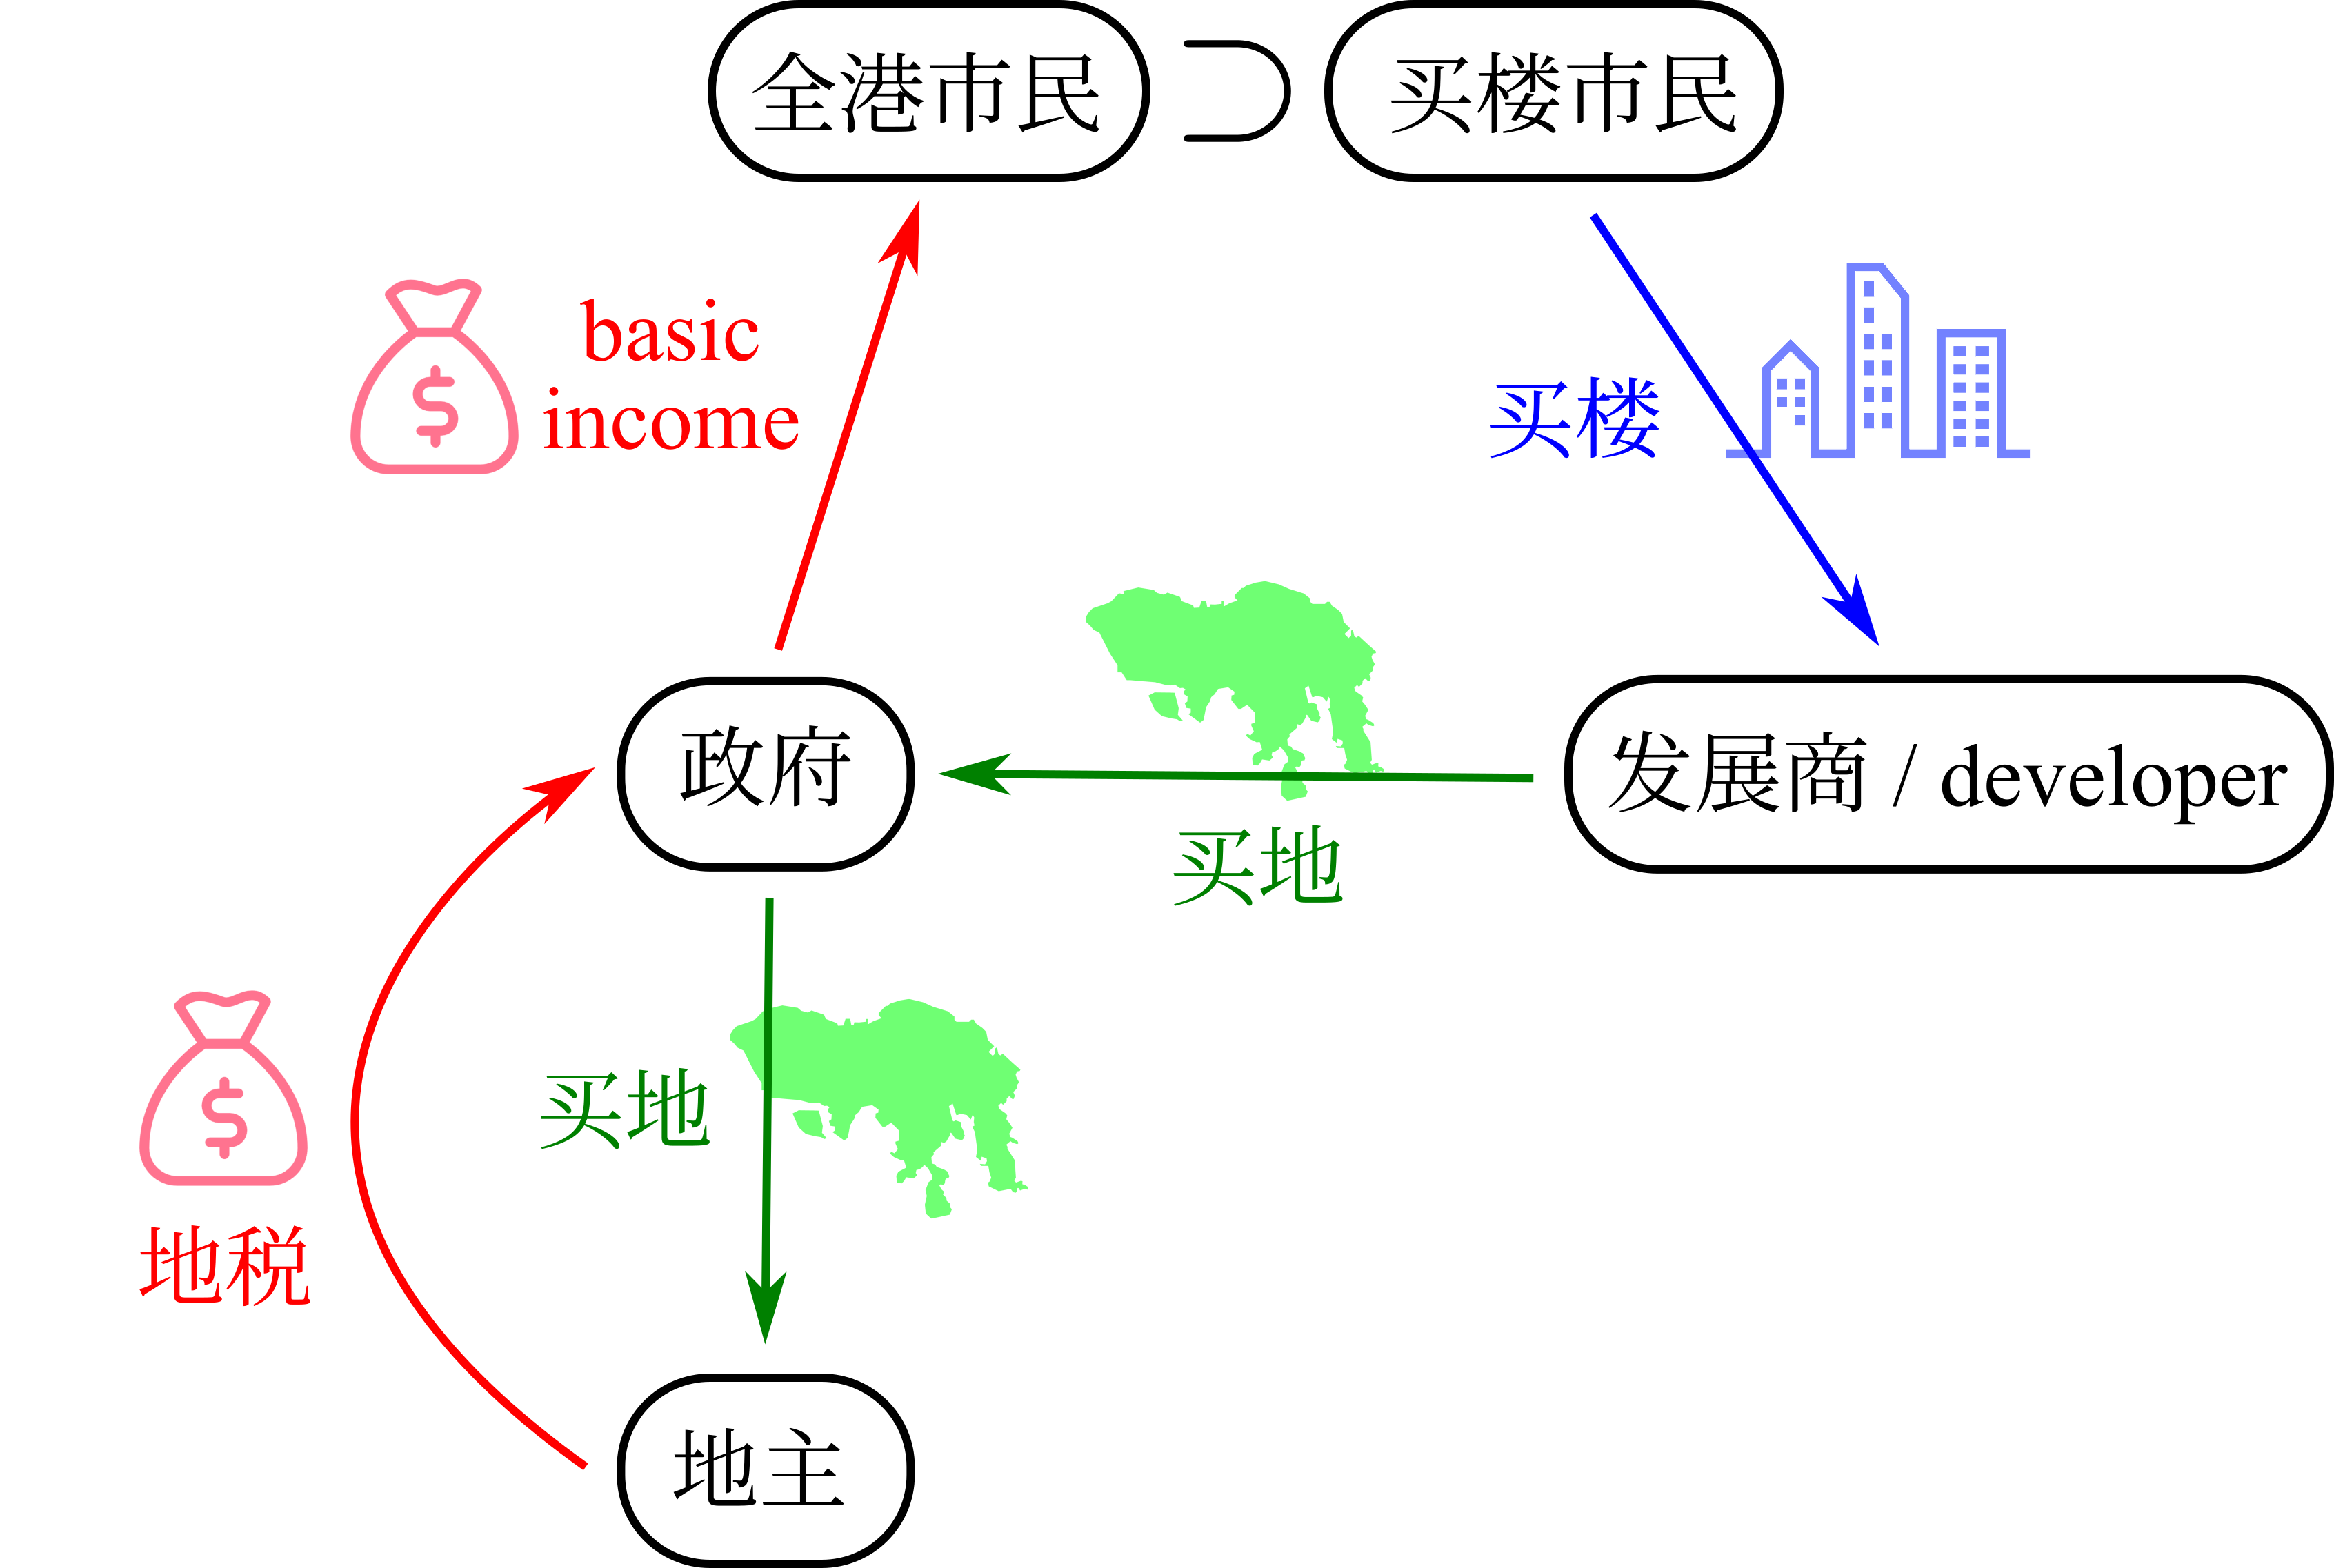
\includegraphics[scale=0.6]{housing-solution.png}}}
\nonumber
\end{equation}
可以考虑 Henry George 提出的: 增加 地税 然后派钱给市民的方案; 《香港地产霸权》的作者 Alice Poon 亦支持这一想法
\end{frame}
\frameinlbffalse

\begin{frame}
\frametitle{土地/房屋 问题 (2)}
传统银行 为商业借贷服务的性质 已经变形; 近年银行体系里,大半的资产 是房地产: 
\begin{equation}
\vcenter{\hbox{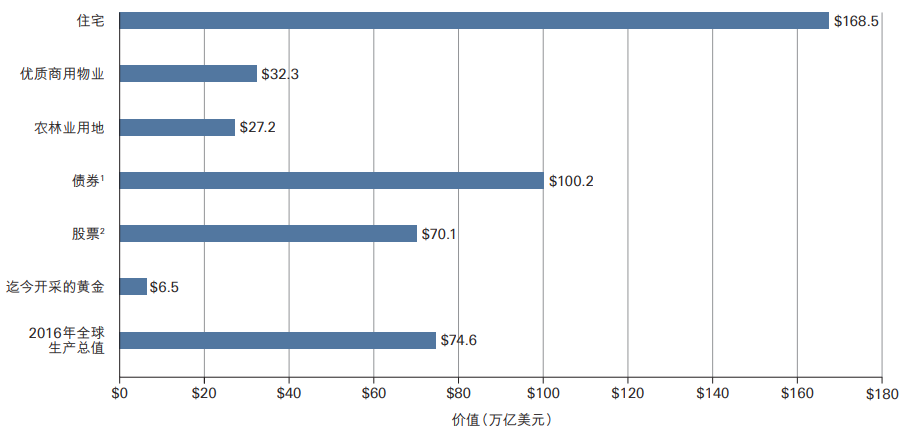
\includegraphics[scale=1.5]{资产类别价值对比-2.png}}}
\nonumber
\end{equation}
中国人喜欢储蓄,大量的财富储存在房地产; 原则上,不应该剥夺人民的私有财产
\end{frame}

\begin{frame}
\frametitle{土地/房屋 问题 (3)}
\begin{itemize}
	\item 在知识型经济下,地产似乎不再是商业发展的樽颈
	
	\item 土地是有限的 \emp{稀缺资源},地产价值不断攀升的情况下,影响高度密集城市的 可持续发展,这是 徵收地税的理由
	
	\item 香港「地产霸权」的形成,很大程度上或许是政府造成,而不是自由市场的错

	\nocite{Ryan-Collins2017}
	\nocite{Farvacque-Vitkoviac1992}
	\nocite{Blomley2004}
	\nocite{Linklater2013}
	\nocite{Adams2015}
	\nocite{简德三2012}
	\nocite{Poon2011}
	\nocite{潘慧娴2010}
	\nocite{OSullivan2012}
	\nocite{Rithmire2015}
	\nocite{Squires2013}
	\nocite{Harvey1996}
	\nocite{Girling1997}
	\nocite{Balia2009}
	\nocite{Peteri2003}
	\nocite{陈云2011}
	\nocite{周其仁2018}
	\nocite{Field2008}
	\nocite{Posner2018}

	\item 在有限的资源下,即使最优的资源分配也无法满足所有人的需要 (wants)

	\item 根据经济学原理,地税 可能会转移给买楼人士; 但似乎可以降低楼价; 不徵税会导致房地产閒置和 投機性 囤积
	
	\item Henry George: \textrm{\textit{``The effect of our present system, which taxes a man for values created by his labor and capital, is to put a fine upon industry, and repress improvement.''}} 他认为应该徵收 land tax 而不是 property tax

	\item 派钱的理据是: 地税的收入应该属於所有香港人,若由政府分配则有低效率和贪腐的问题
	
	\item 现时,公屋的挑选要求「低收入」不合理,破坏香港人上进的动机,而且抽签 产生「听天由命」心态

	% \item Rent-seeking 不是 land tax 的理由,但稀缺资源是

	% \item 如是者,则 land tax 的目的,必然是将稀缺资源作公平分配

	% \item 问题是 land tax 要收到什么程度?  也许,直到 平均收入 追得上为止。

	% \item 但地税 会 transfer 给租户和住户,导致 楼价 仍然高企。  这样则进一步 增加 basic income.
\end{itemize}
\end{frame}

\frameinlbftrue
\begin{frame}
\frametitle{医疗}
\begin{itemize}
	\item 香港 公立医院 对医护人员的待遇苛刻,「慷他人之慨」,迎合市民贪便宜的心态,实则对公众不利
	
	\item 公立医院 收费过廉,导致 私家医院 被逼提高收费,造成市场上高低两端的「断裂」,和楼市的情况一样
	
	\item 医疗的进步,并不在於廉价劳工,而是需要 技术的进步,包括投入资金 进行 R\&D
	
	\item 政府对医疗的管制其实妨碍了医疗技术的发展
	
	\item 现时在医院死亡的首要原因是医疗失误
\end{itemize}
\end{frame}

\begin{frame}
\frametitle{教育}
\begin{itemize}
	\item 香港 填鸭式教育 已被批评到老掉牙
	
	\item 实际上 香港各大学内,课程、课本、设施等,都和外国大学几乎一模一样
	
	\item 问题是香港(和亚洲很多国家一样)高等教育的普及程度不足
	
	\item 在西方,一般人想读大学 基本上可以找到学位,但香港则「争崩头」 
	
	\item 在「争崩头」情况下,学生/研究生们 专注於争取分数/排名,忘记了求学问的初心 
	
	\item 免费而高质素的网上课程很多,但香港人不重视学问,因为 ``high tech 揩嘢,low tech 捞嘢'' 的环境造成
	
	\item 香港有高科技 R\&D 的公司几乎不存在,没有企业将科技的利润 \emp{回馈} 到学术界,教育的 positive feedback loop 断开了,这情况和外国没有可比性,不能照搬外国的教育制度
	
	\item 資源平均分配 給所有香港人,比 在排名上追上外國大學標準 更重要
	
	\item 同样地,政府应该「放手」让教育自由化
	
	\item 在《城市論壇》中經常有聽眾不夠時間發言的情況,可以 建立多些空間 增加市民發言/討論 的機會
\end{itemize}
\end{frame}

\frame[allowframebreaks]{
多谢收看 \smiley
% \frametitle{References}
\printbibliography
}

\begin{frame}
\frametitle{关於我}
\fontsize{7pt}{7.2}\selectfont
	\begin{columns}[T]
		\begin{column}{0.65\textwidth}
		\begin{itemize}
			\item 1971年 生於香港
			\item 父亲是殖民时期警察,升至高级警司,受过 彭定康 颁奖,回归后不久退休
			\item 母亲家庭主妇
			\item 北角卫理小学
			\item 金文泰中学,圣保罗男女中学
			\item 我年轻时经常看很多大陆出版的科学、数学、文史哲书,我好细个已经识读同写简体字
			\item 在 70-80 年代,简体字书很平,我对简体字很有亲切感,当时我买不起英文书籍,只有很少几本
			\item 我用简体字是因为觉得简体字靓,同政治冇关,这一点已经解释过好多次
			\item 本人亦很喜欢中国书法,最锺意《古诗四帖》
		\end{itemize}
		\end{column}

		\begin{column}{0.35\textwidth}
		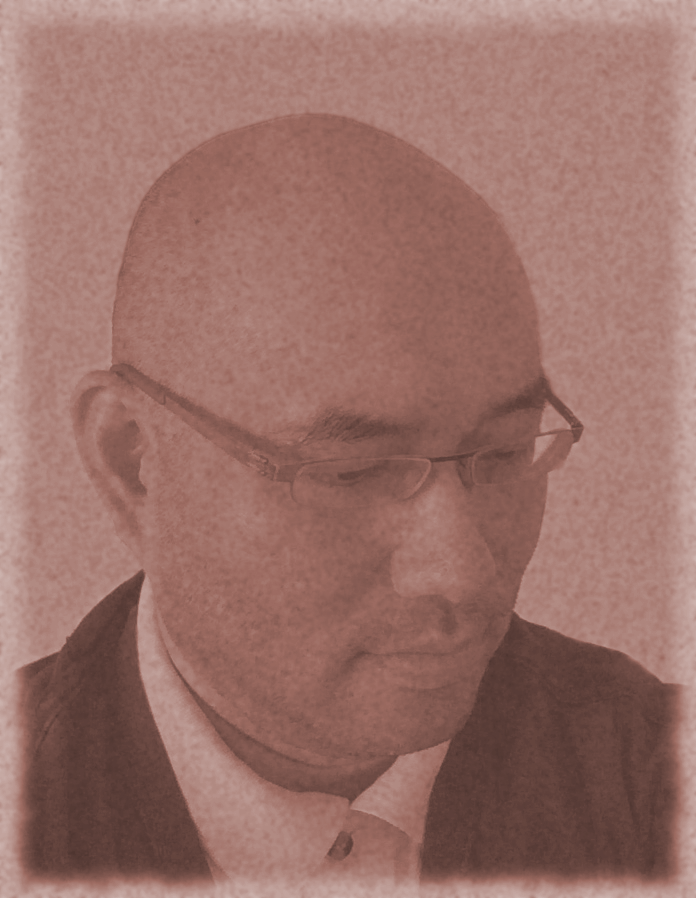
\includegraphics[scale=0.15]{../John_Grothendieck.png}
		\end{column}
	\end{columns}

	\begin{itemize}
		\item 香港中文大学,主修电脑,后转读艺术,但因学分太低被踢鸠咗出嚟
		\item 我在 人工智能 这科拿了个 F,只上过一两堂,唔记得咗去考试
		\item 我在中大时 浑浑噩噩,对金钱没有兴趣,但有不少朋友
		\item 暑假时,美国的堂妹来港,嘲笑我係香港人落后,我好唔开心
		\item 去了美国 纽约的 Hofstra 大学,主修 会计、英美文学、生物化学 等
		\item 留学美国之后我感到很自卑,於是发奋读书
		\item 政治上我初时左倾,后来变 libertarian,性格上亦变得很进取,谁知回到香港后冇晒朋友,跟香港人格格不入
	\end{itemize}
\end{frame}

\begin{frame}[plain]
	\begin{itemize}
		\item 
	\end{itemize}
\end{frame}

\end{document} 